\documentclass{article}
\usepackage[utf8]{inputenc}
\usepackage[italian]{babel}
\usepackage{graphicx}


\usepackage{epstopdf}


%\usepackage{floatrow}%
%\usepackage{algpseudocode}
%\usepackage[ruled,noline,linesnumbered]{algorithm2e}


%texttt line break trick
%\usepackage{lipsum}
%
%\newcommand*\justify{%
%  \fontdimen2\font=0.4em% interword space
%  \fontdimen3\font=0.2em% interword stretch
%  \fontdimen4\font=0.1em% interword shrink
%  \fontdimen7\font=0.1em% extra space
%  \hyphenchar\font=`\-% allowing hyphenation
%}

%margins
%\usepackage[margin=2cm]{geometry}


\let\emptyset\varnothing


\graphicspath{ {./images/} }

\title{La Speranza è una Trappola}
\author{Federico D'Amato, Alessio Sarullo}

\begin{document}
\maketitle

% \tableofcontents
% \newpage

\section{Introduzione}
L'obiettivo di questo elaborato è quello di modellare e simulare il problema di \textit{bus arbitration}, utilizzando il protocollo Linear Two-Phase Commit. Lo scenario è quello in cui \textit{n} processori fanno periodiche richieste di accesso ad un bus qualunque tra un insieme di \textit{m} disponibili.\\
Ogni processore ed ogni bus viene modellato tramite una macchina a stati finiti; il tool utilizzato per la realizzazione di tali macchine è SMCube, della suite Scicos. L'intero sistema è rappresentato da un insieme di macchine a stati finiti realizzati con SMCube e da un certo numero di blocchi funzionali propri dell'ambiente Scicos, interconnessi fra loro.\\
Nella prima parte della relazione viene descritto il tool SMCube, sia dal punto di vista dell'interfaccia utente, sia da quello delle funzionalità offerte. Successivamente, il problema di \textit{bus arbitration} viene descritto nel dettaglio, così come gli obiettivi dell'elaborato ed i vincoli realizzativi. Nella sezione successiva vengono mostrate le implementazioni delle macchine a stati (processori e bus) e del sistema di interconnessione risultante. Infine vengono illustrate le simulazioni effettuate, cercando di evidenziare eventuali punti di forza o debolezze dell'approccio realizzativo utilizzato.

\section{SMCube}
SMCube\cite{smcube} è un tool per la modellazione, simulazione e generazione di codice per automi a stati finiti (\textsl{ASF}) a tempo discreto. È stato progettato per essere integrato all'interno del framework \textsl{Scicos}\cite{scicos}, permettendo la creazione di data-flow diagram che contengono ASF. In questo modello ibrido, i componenti del data-flow diagram vengono usati per gestire il flusso dei dati, mentre gli automi a stati finiti vengono usati per aggiungere comportamenti più complessi, non facilmente implementabili altrimenti.

Nelle sezioni seguenti verrà data un'idea generale dell'applicazione. Per maggiori dettagli si rimanda a \cite{smcube_man}.

\subsection{Modellazione di un ASF tramite SMCube}
In SMCube la modellazione di un ASF avviene per via grafica. Le figure \ref{Fig:smcube_ex_init} e \ref{Fig:smcube_ex_state} mostrano, rispettivamente, lo stato iniziale e uno stato generico dell'automa, mentre in figura \ref{Fig:smcube_ex_transition} viene mostrata una transizione tra due stati.

Il tempo all'interno di SMCube è discreto ed è scandito dal verificarsi di \textsl{eventi}. L'integrazione con Scicos consente di definirne uno solo, che nel nostro caso è un clock comune a tutti i nodi. Al verificarsi dell'evento viene effettuata la transizione eseguibile con la priorità più alta, o si permane nello stato attuale se non ci sono transizioni eseguibili.

Nella modellazione di una macchina a stati con SMCube esiste la possibilità di definire delle \textsl{azioni}. L'esecuzione delle azioni può avvenire con diverse modalità:

\begin{itemize}
\item durante una transizione
\item entrando in uno stato
\item permanendo in uno stato
\item uscendo dallo stato.
\end{itemize}

Le azioni consentono di inviare segnali in output o modificare i valori delle variabili locali; questi valori, insieme agli input ricevuti, possono poi essere utilizzati all'interno delle \textsl{guardie}, che permettono di controllare l'esecuzione delle transizioni. In figure \ref{Fig:smcube_ex_ga} è mostrato un esempio di azioni e guardie che fanno utilizzo sia delle variabili locali che dei segnali inviati e ricevuti.

%\newcommand{\csubfloat}[2][]{%
%  \makebox[0pt]{\subfloat[#1]{#2}}%
%}
%\newcommand{\centerhfill}[1][\quad]{\hspace{\stretch{0.5}}#1\hspace{\stretch{0.5}}}
%\begin{figure}
%\centering
%\csubfloat[Stato iniziale di un ASF in SMCube. \label{Fig:smcube_ex_init}]
%	{\makebox[.3\textwidth][c]{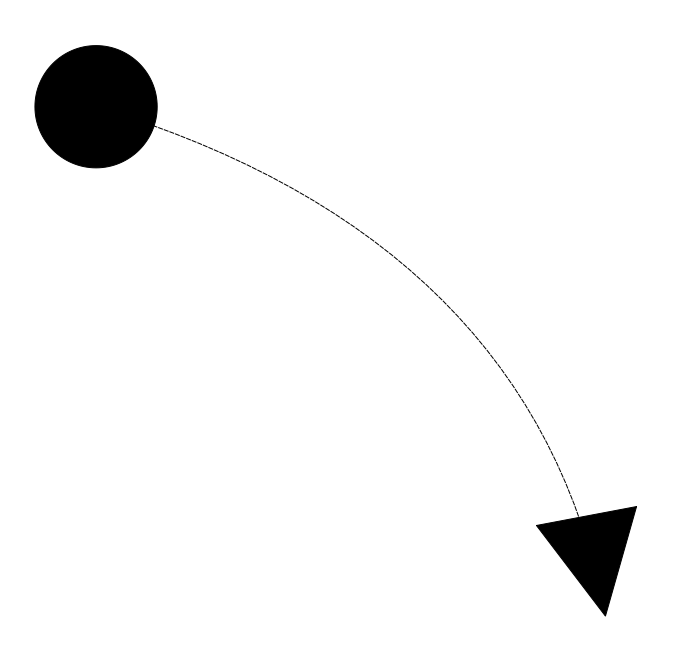
\includegraphics[width=0.1\textwidth]{smcube_ex_init.png}}}\centerhfill
%\csubfloat[Un generico stato in SMCube. \label{Fig:smcube_ex_state}]
%	{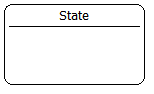
\includegraphics[width=0.3\textwidth]{smcube_ex_state.png}}\centerhfill
%\csubfloat[Transizione di priorità 1 dallo stato \texttt{State\_1} allo stato \texttt{State\_2} in SMCube. \label{Fig:smcube_ex_transition}]
%	{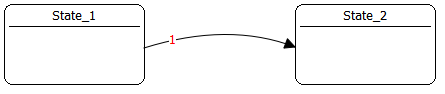
\includegraphics[width=0.5\textwidth]{smcube_ex_transition.png}}
%\caption{Componenti fondamentali di SMCube}
%\label{Fig:smcube_blocks}
%\end{figure}

\begin{figure}
\makebox[\textwidth][c]{
	\begin{subfigure}[t]{.3\textwidth}
		\centering
		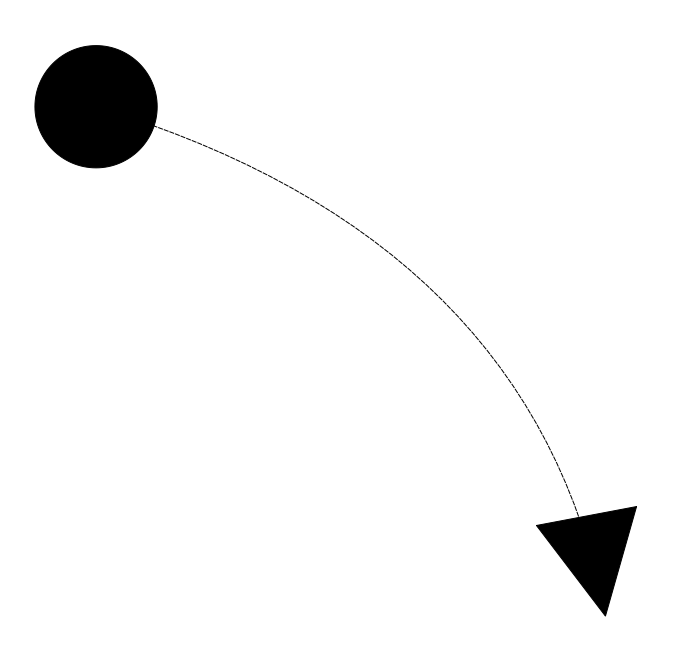
\includegraphics[width=.3\textwidth]{smcube_ex_init.png}
		\caption{Stato iniziale.}
		\label{Fig:smcube_ex_init}
	\end{subfigure}
	
	\begin{subfigure}[t]{.3\textwidth}
		\centering
		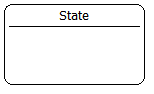
\includegraphics[width=.8\textwidth]{smcube_ex_state.png}
		\caption{Stato generico.}
		\label{Fig:smcube_ex_state}
	\end{subfigure}
	
	\begin{subfigure}[t]{.7\textwidth}
		\centering
		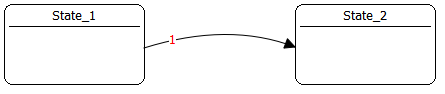
\includegraphics[width=.95\textwidth]{smcube_ex_transition.png}
		\caption{Transizione di priorità 1 dallo stato \texttt{State\_1} allo stato \texttt{State\_2}.}
		\label{Fig:smcube_ex_transition}
	\end{subfigure}%
}
\caption{Componenti fondamentali di un ASF in SMCube.}
\label{Fig:smcube_blocks}
\end{figure}

\begin{figure}
\centering
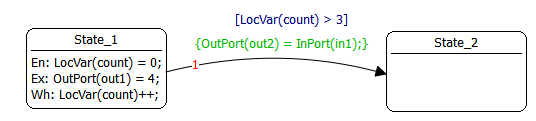
\includegraphics[width=1\textwidth]{smcube_ex_ga.png}
\caption{Esempio di azioni e guardie. Le label \textit{en}, \textit{ex} e \textit{wh} indicano rispettivamente le azioni compiute entrando, uscendo o permanendo nello stato. Sulla transizione sono presenti una guardia (in blu, tra parentesi quadre) e un'azione (in verde, tra graffe). Le keyword \texttt{LocVar}, \texttt{OutPort} e \texttt{InPort} consentono di far riferimento rispettivamente a variabili locali, porte di output e porte di input.}
\label{Fig:smcube_ex_ga}
\end{figure}

\subsection{Integrazione con Scicos}
Scicos è un modellatore grafico, simulatore e generatore di codice per sistemi dinamici. Un diagramma Scicos è costituito da una serie di blocchi comunicanti tra loro attraverso due tipi di porte: dati ed eventi. I dati costituiscono le informazioni di interesse che vengono manipolate dai vari blocchi, mentre gli eventi sono usati per comunicare ad un blocco quando eseguire determinate azioni. In figura \ref{Fig:scicos_ex} è mostrato un esempio di diagramma Scicos.\\

\begin{figure}
\centering
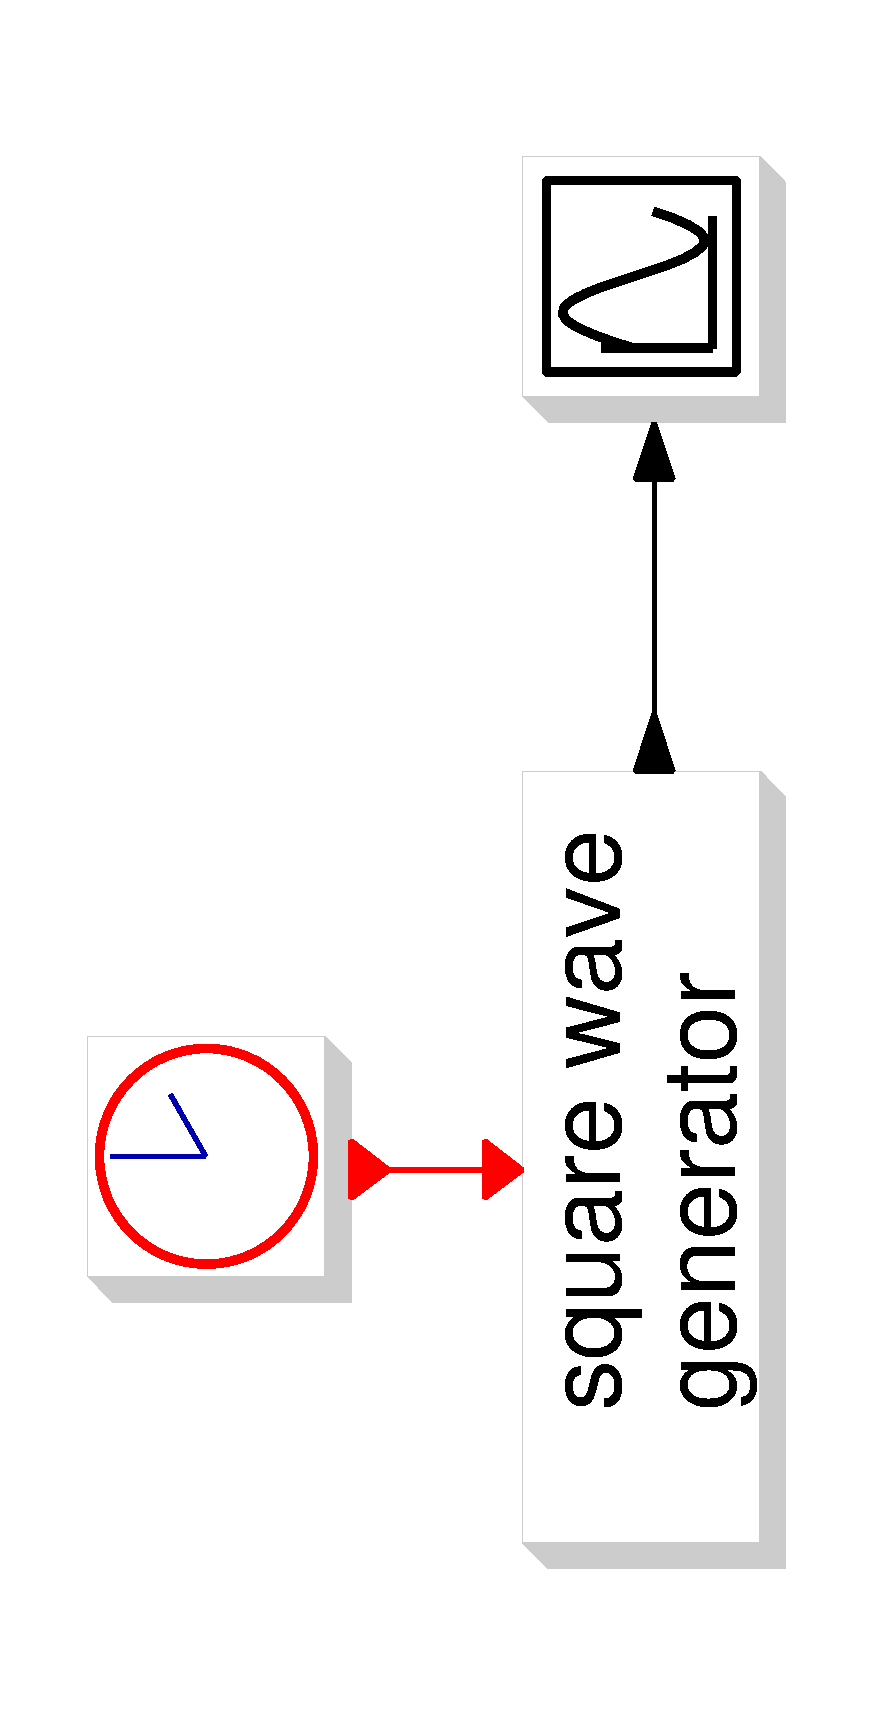
\includegraphics[angle=-90, width=0.35\textwidth]{scicos_ex.eps}
\caption{Un diagramma Scicos che stampa a video un'onda quadra. In rosso sono rappresentati i collegamenti e le porte relativi agli eventi, in nero quelli relativi ai dati. Ad ogni colpo di clock il generatore esegue un'azione, cambiando il valore in output. Il risultato è un'onda quadra con periodo pari a 2 colpi di clock.}
\label{Fig:scicos_ex}
\end{figure}

L'integrazione di ASF progettati con SMCube all'interno di diagrammi Scicos è molto semplice: è sufficiente inserire un blocco SMCube all'interno del diagramma e specificare il file in cui è stato definito l'automa a cui il blocco si riferisce, come mostrato in figura \ref{Fig:smcube_scicos_ex}. Una volta integrato il blocco, è possibile eseguire la simulazione in due modalità: batch e interattiva. La modalità batch è efficiente, ma non produce output ed è quindi più indicata per eseguire la simulazione dell'intero modello, assumendo che l'ASF rappresentato dal blocco sia corretto. La modalità interattiva, invece, produce un output grafico e consente anche un'esecuzione step-by-step, al costo ovviamente della velocità di esecuzione; è pertanto più indicata per eseguire il debug dell'ASF o anche dell'intero sistema, perché consente di controllare i dati che arrivano all'automa, il sui stato interno o gli output che esso produce.

\begin{figure}
\centering
\makebox[\textwidth][c]{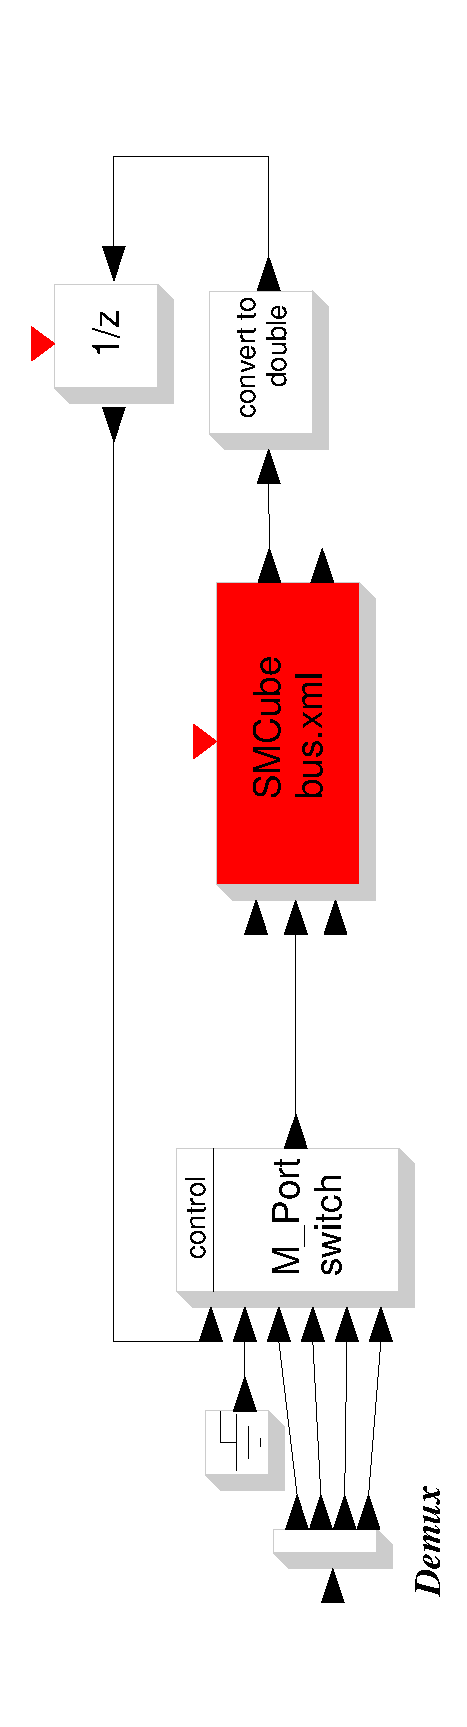
\includegraphics[angle=-90, width=1.2\textwidth]{smcube_block_ex.eps}}%
\caption{Blocco SMCube rappresentante un bus (in rosso) all'interno di un diagramma Scicos.}
\label{Fig:smcube_scicos_ex}
\end{figure}
\section{Descrizione del problema}
Il problema in esame è quello di \textit{bus arbitration}, problema tipico in ambienti multi-processore. Il caso è quello in cui $n$ processori ${p_1,..,p_n}$  fanno periodiche richieste di accesso ad uno qualunque degli $m$ bus fra ${b_1,..,b_m}$. In un qualsiasi istante di tempo, un bus è assegnato al più ad un processore ed un processore sta utilizzando al più un unico bus.\\
In Figura \ref{Fig:uml} sono mostrate delle macchine a stati finiti che modellano, in prima approssimazione, il comportamento di processori e bus. Un processore invia un segnale di \textit{request} per richiedere l'accesso ad un bus. Se la richiesta ha buon fine, usa il bus fino a quando decide di rilasciarlo (segnale \textit{release}). Il controllore del bus ha un comportamento speculare: a seguito di una richiesta manda un segnale di \textit{grant} al processore, aspettando un segnale di avvenuta ricezione (\textit{ack}), e poi attende che il processore lo rilasci.\\
Rispetto alle macchine a stati di Figura \ref{Fig:uml}, si rende necessaria la realizzazione di un meccanismo che garantisca l’unicità della segnalazione di \textit{grant} per una coppia processore-bus. Inoltre deve essere possibile, in un dato istante, riconoscere l’impossibilità temporanea di servire un processore e poter segnalare questa situazione al processore richiedente con un segnale di \textit{nack}.\\
Nel caso di più richieste di utilizzo di uno stesso bus da parte di processori distinti, si pone anche il problema di decidere a quale processore assegnare il bus. Vengono prese in esame due diverse politiche di gestione:
\begin{itemize}
\item Equal priority:  tutti i processori hanno la stessa priorità ed evenutali richieste in conflitto vengono servite in ordine FIFO di arrivo
\item Fixed priority:  i processori hanno una diversa priorità e in caso di richieste "simultanee" (nello stesso ciclo di clock) si serve quella del processore prioritario
\end{itemize}
\begin{center}
\begin{figure}
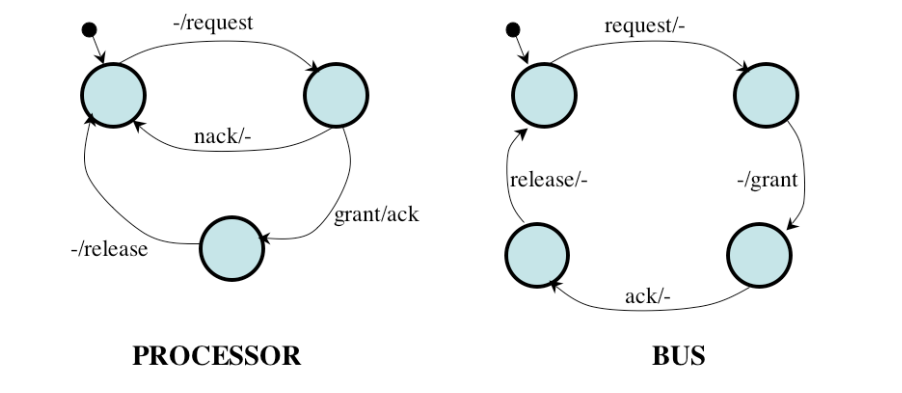
\includegraphics[scale=0.6]{uml_processor_bus}
\caption{Schemi funzionali di processori e bus}
\label{Fig:uml}
\end{figure}
\begin{figure}
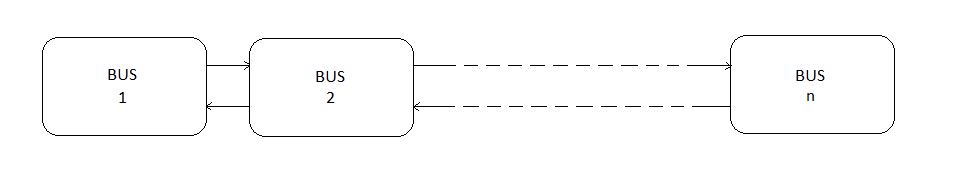
\includegraphics[scale=0.6]{2pc}
\caption{Collegamento a catena dei bus}
\label{Fig:2pc}
\end{figure}
\end{center}
Per la generazione dei segnali di \textit{grant} e \textit{nack}, i nodi bus eseguono il protocollo \textit{Two-Phase Commit} in versione lineare. In questa versione del protocollo, i nodi bus sono collegati a catena, come in Figura \ref{Fig:2pc}. Ogni partecipante ha un numero progressivo e conosce il precedente e il successivo; l'ultimo nodo della catena sa di essere l'ultimo. Il protocollo procede attraverso due fasi successive:
\begin{itemize}
\item Fase 1: ogni nodo, partendo dal primo fino all'ultimo, comunica di essere arrivato al punto di \textit{commit} (o \textit{abort} nel caso qualcosa non abbia funzionato)
\item Fase 2: l'ultimo nodo risponde \textit{OK} e il messaggio percorre in senso inverso la catena
\end{itemize}
Una realizzazione alternativa del protocollo prevede un collegamento aggiuntivo tra l'ultimo elemento della catena ed il primo; in questo caso la topologia diventa ad \textit{anello} e il protocollo rimane sostanzialmente invariato.
\subsection{Caso specifico}
In questo elaborato viene realizzato un sistema con $n=4$ processori ed $m=3$ bus. Sul modello risultante, viene richiesto di verificare tramite simulazione le seguenti proprietà:
\begin{itemize}
\item Safety: mutua esclusione nell'accesso ai bus
\item Liveness: assenza di \textit{livelock}, cioè di computazioni nelle quali un processore ripete indefinitamente richieste di accesso che non vengono mai servite
\item Liveness: assenza di \textit{deadlock}, ovvero di computazioni in cui un processore non è in grado di accedere al bus perché il protocollo non garantisce di completare la comunicazione
\end{itemize}

\section{Implementazione}
Il modello descritto nella sezione \ref{Sec:problem} è stato realizzato tramite un diagramma Scicos, utilizzando SMCube per modellare processori, bus e coordinatore dei bus. In figura \ref{Fig:model_ep} è mostrato il diagramma relativo al caso Equal Priority, mentre la figura \ref{Fig:model_fp} rappresenta il modello Fixed Priority. Ovviamente, i due modelli sono del tutto identici a parte per come viene gestita la coda delle richieste che arrivano al coordinatore.

\begin{figure}
\vspace{-3cm}
\centerline{
	\begin{subfigure}[t]{1.4\textwidth}
		\centering
		\includegraphics[angle=-90, width=\textwidth]{model_ep.eps}
		\caption{Diagramma del modello Equal Priority.}
		\label{Fig:model_ep}
	\end{subfigure}
}
\centerline{
	\begin{subfigure}[t]{1.4\textwidth}
		\centering
		\includegraphics[angle=-90, width=\textwidth]{model_fp.eps}
		\caption{Diagramma del modello Fixed Priority.}
		\label{Fig:model_fp}
	\end{subfigure}
}
\caption{I due modelli implementati: Equal Priority \subref{Fig:model_ep} e Fixed Priority \subref{Fig:model_fp}. In grigio sono evidenziati i blocchi che costituiscono la coda di priorità.}
\label{Fig:models}
\end{figure}

È importante evidenziare due decisioni di progetto che sono state prese nella rappresentazione del modello:

\begin{enumerate}
\item \textbf{Disporre i bus secondo una topologia ad anello orientato}. Il motivo di questa scelta deriva da un controllo che Scicos effettua in fase di compilazione del modello per rilevare \textsl{loop algebrici}, ossia cicli di input e output potenzialmente infiniti che portano al fallimento della simulazione (figura \ref{Fig:alg_loop}). È quindi necessario aggiungere un elemento di ritardo qualora due blocchi debbano comunicare reciprocamente (o un blocco utilizzi una sua risposta come input, come accade nell'esempio di figura \ref{Fig:alg_loop_solved}). Questo significa che, nel caso di una struttura lineare come quella mostrata in figura \ref{Fig:2pc}, ogni messaggio della seconda fase del protocollo subirebbe un ritardo di un colpo di clock, rendendo la complessità temporale del protocollo lineare rispetto al numero di nodi. Con una struttura ad anello orientato, invece, occorre inserire un blocco ritardo soltanto tra due bus. La configurazione ottimale prevede il ritardo tra l'ultimo bus dell'anello (ossia quello che precede il coordinatore del 2PC) ed il coordinatore: così facendo, in un colpo di clock viene deciso quale bus soddisferà la richiesta e nel secondo colpo di clock viene raggiunta conoscenza comune.
\item \textbf{Separare la logica del coordinatore del 2PC da quella dei bus}. In questo modo tutti i bus hanno lo stesso comportamento, evitando di dover differenziare la logica del bus coordinatore da quella degli altri. Inoltre, l'automa a stati finiti di un coordinatore \textquotedblleft semplice\textquotedblright{} è ovviamente meno complesso di quello di un coordinatore che è anche un bus, diminuendo quindi la possibilità di errori in fase di implementazione. Il costo da pagare è soltanto l'aggiunta del nodo coordinatore all'interno dell'anello dei bus.
\end{enumerate}

\begin{figure}
\makebox[\textwidth][c]{
	\begin{subfigure}[t]{.5\textwidth}
		\centering
		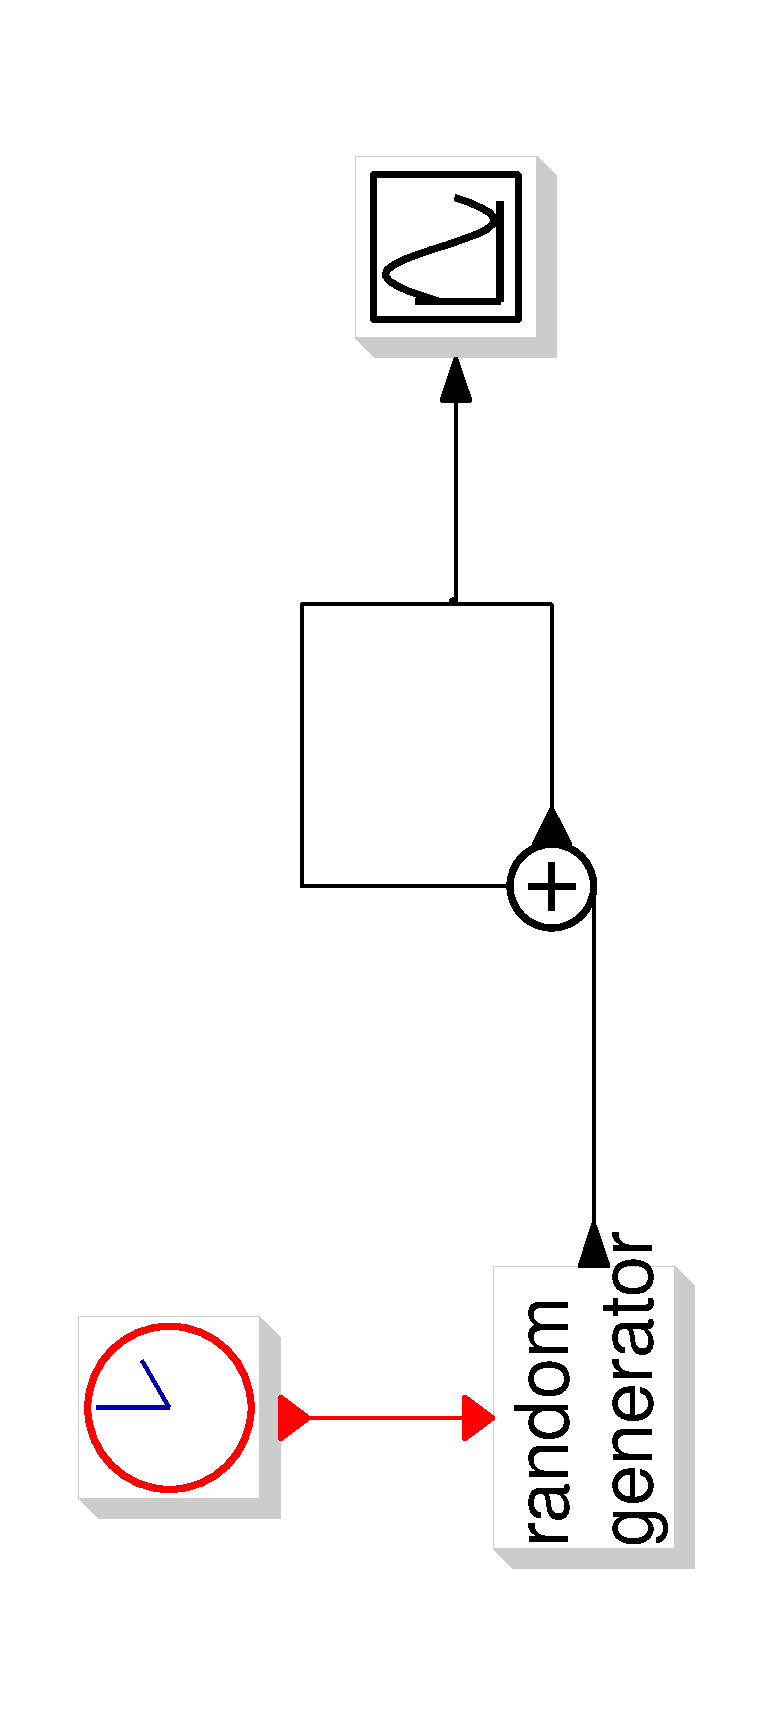
\includegraphics[angle=-90, totalheight=.45\textwidth]{alg_loop.eps}
		\caption{}
		\label{Fig:alg_loop}
	\end{subfigure}
	
	\begin{subfigure}[t]{.5\textwidth}
		\centering
		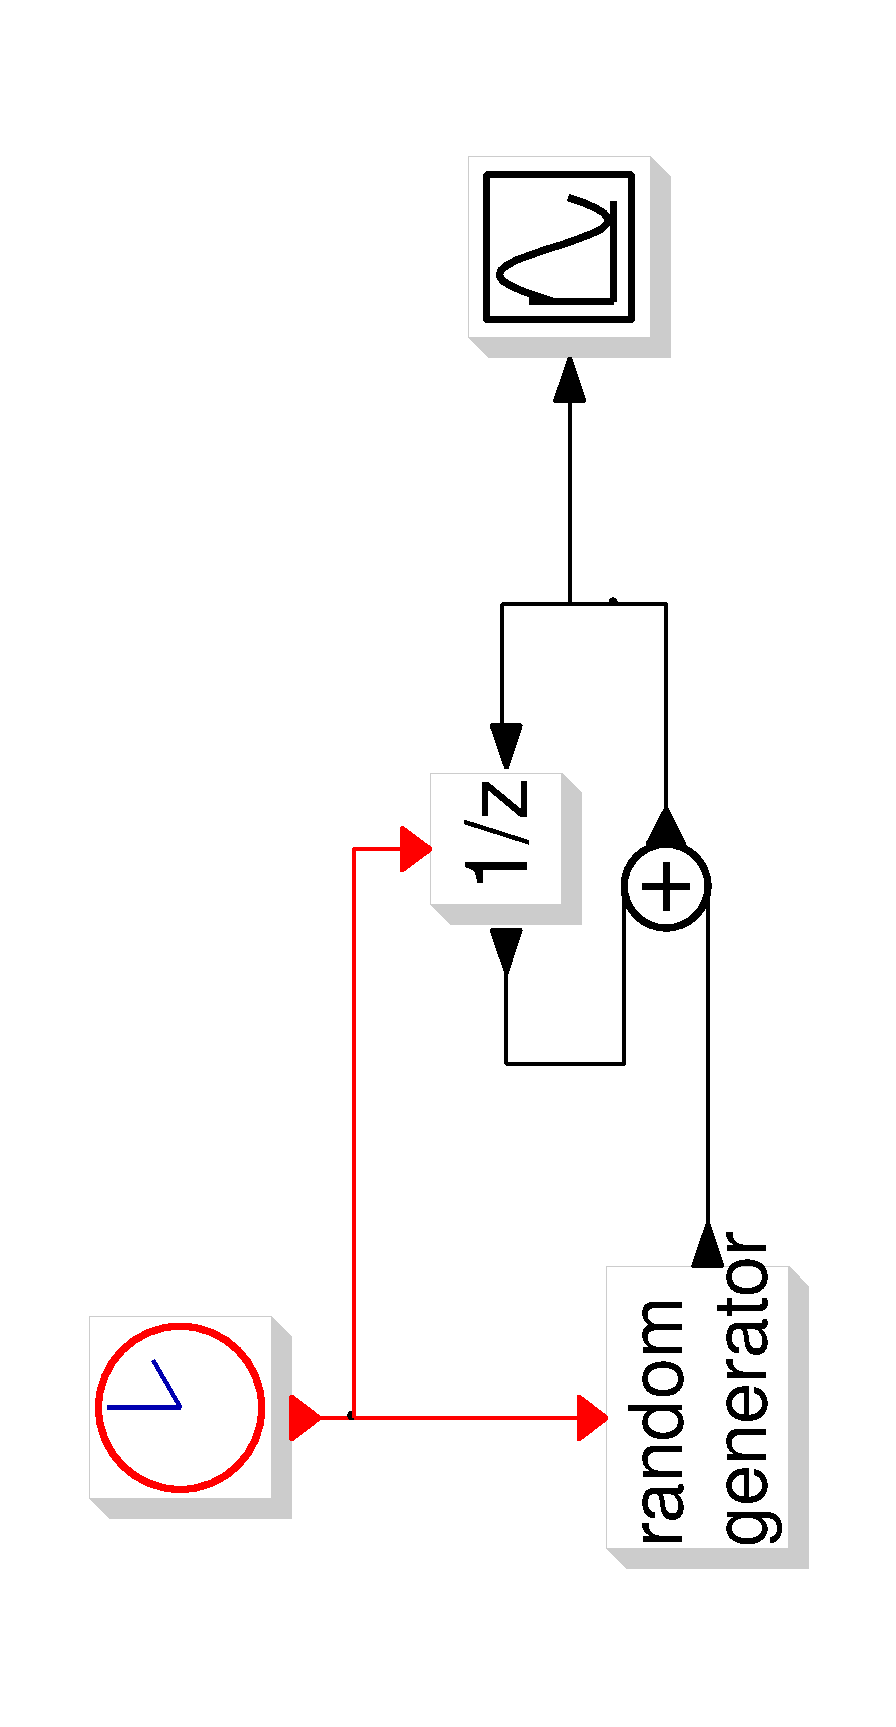
\includegraphics[angle=-90, totalheight=.45\textwidth]{alg_loop_solved.eps}
		\caption{}
		\label{Fig:alg_loop_solved}
	\end{subfigure}
}
\caption{La figura \subref{Fig:alg_loop} mostra un diagramma Scicos che contiene un loop algebrico, mentre in figura \subref{Fig:alg_loop_solved} è raffigurato un diagramma equivalente che risolve il problema inserendo un blocco ritardo.}
\label{Fig:loops}
\end{figure}

\noindent
Il modello è costruito per via grafica ed è abbastanza autoesplicativo: è facile vedere come i processori, il coordinatore ed i bus sono collegati tra di loro. Vale la pena però porre l'attenzione sugli switch antecedenti ai bus che filtrano gli output dei processori. Mentre per effettuare la richiesta i processori comunicano di fatto solo con il coordinatore, una volta garantito l'accesso la comunicazione con i bus avviene per via diretta, per evitare di aggiungere ulteriore carico di lavoro al coordinatore e rallentare le comunicazioni. Questo vuol dire che tutti i processori sono collegati a tutti i bus, ma \textit{non} è vero che tutti i segnali inviati dai processori arrivano a tutti i bus: ogni bus, infatti, controlla il proprio switch in modo che solo i segnali inviati dal processore che ha l'accesso possano arrivare.\\

Nel seguito descriveremo gli automi che modellano i processori, i bus e il coordinatore dei bus.

\subsection{Processore} 
L'automa del processore è riprodotto in figura \ref{Fig:proc_fsm}. È funzionalmente equivalente a quello riportato nelle specifiche e mostrato in figura \ref{Fig:uml}. Da notare che il tempo di soggiorno negli stati \texttt{Idle} e \texttt{Using} è random e viene campionato al momento dell'entrata nello stato.

\begin{figure}[!hb]
%\vspace{-1cm}
\centerline{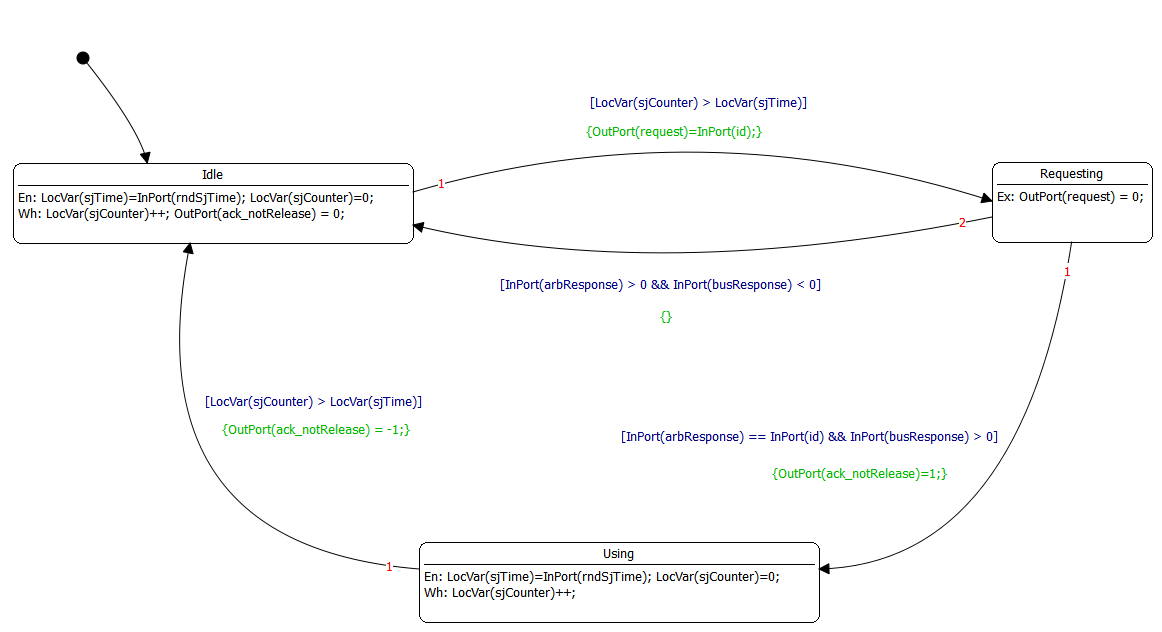
\includegraphics[width=1.4\textwidth]{processor.png}}
\caption{ASF di un processore.}
\label{Fig:proc_fsm}
\vspace{-2cm}
\end{figure}

\subsection{Coordinatore dei bus} 
L'automa del coordinatore viene mostrato in figura \ref{Fig:coord_fsm}. È composto da tre stati:

\begin{itemize}
\item \texttt{Idle}: il coordinatore è in attesa di richieste da parte dei processori.
\item \texttt{NotifyingBuses}: è arrivata una richiesta ed è stata inoltrata ai bus, dando via alla prima fase del 2PC. Il coordinatore è in attesa di sapere quale bus ha accolto la richiesta.
\item \texttt{Committing}: la richiesta è passata per tutti i bus dell'anello, tornando al coordinatore. Questo significa che a tutti i bus è arrivata la notifica della richiesta e sono tutti in attesa del commit. Il messaggio che arriva al coordinatore contiene l'id del bus che soddisferà la richiesta (o -1 se non ci sono bus disponibili) e il coordinatore non deve fare altro che inoltrarlo sia ai bus che ai processori. Quando il messaggio percorre tutto l'anello e ritorna al coordinatore, tutti i bus e i processori sono stati notificati del risultato della richiesta e il coordinatore può tornare nello stato di \texttt{Idle}.
\end{itemize}

\begin{figure}[!hb]
\vspace{-.5cm}
\centerline{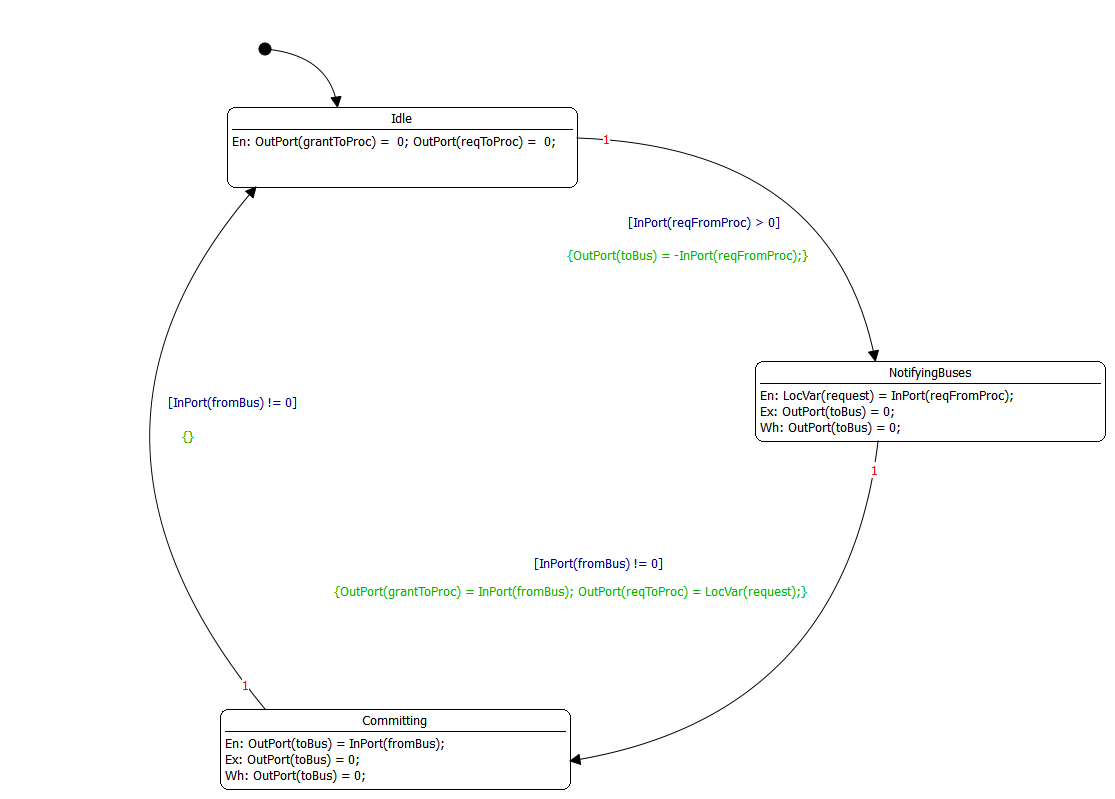
\includegraphics[width=1.3\textwidth]{busCoord.png}}
\caption{ASF del coordinatore dei bus.}
\label{Fig:coord_fsm}
\vspace{-2cm}
\end{figure}

\pagebreak

\subsection{Bus} 

\begin{figure}[t]
\vspace{-2cm}
\centerline{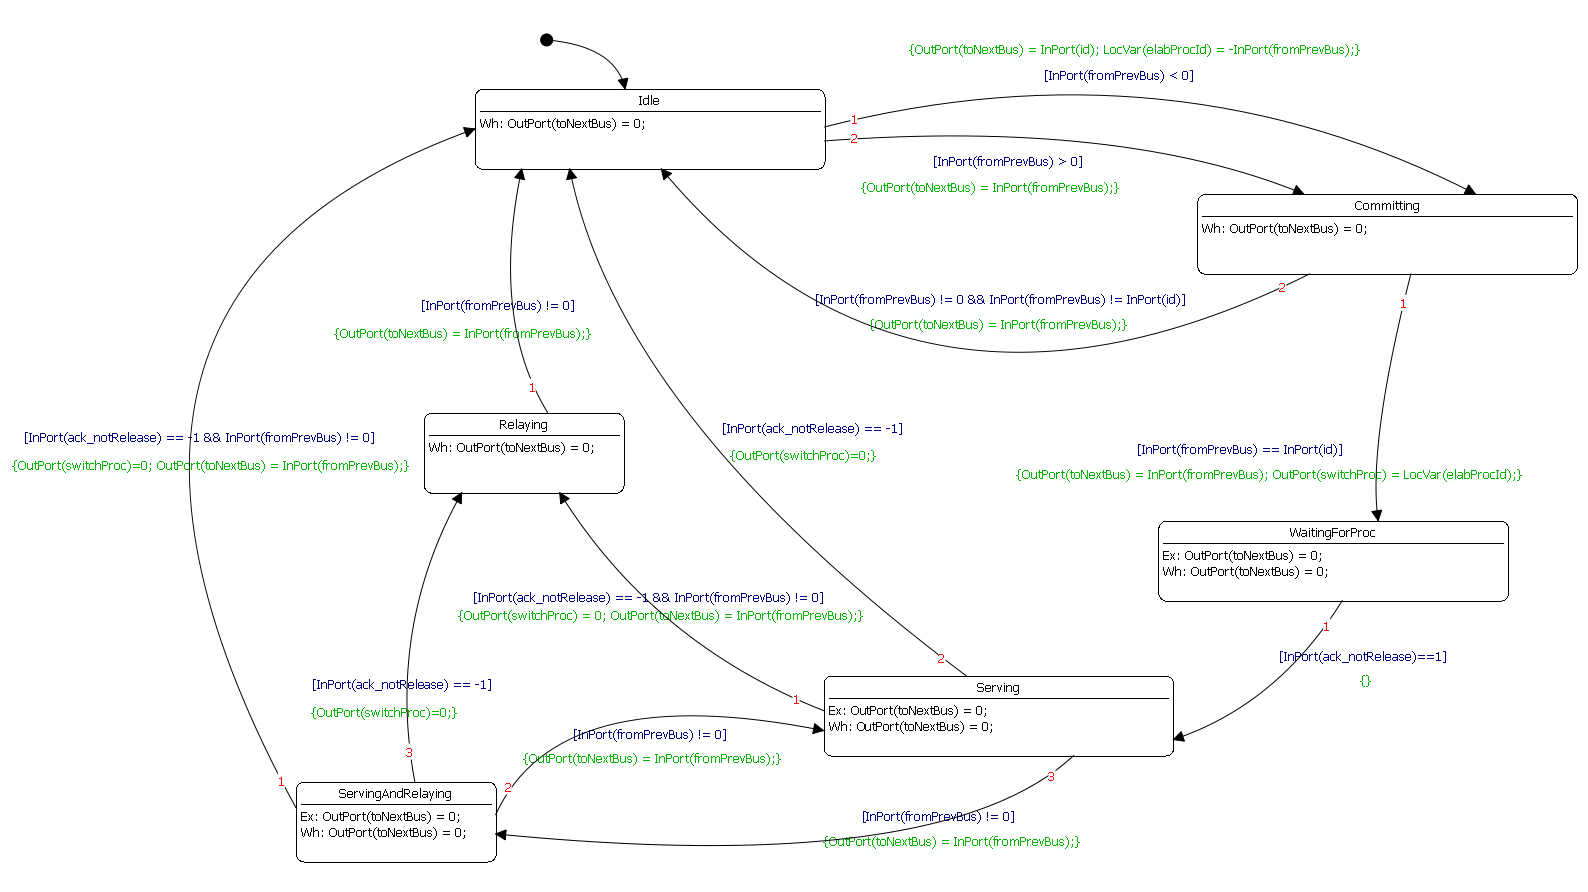
\includegraphics[width=1.6\textwidth]{bus.png}}
\caption{ASF dei bus.}
\label{Fig:bus_fsm}
\end{figure}

I bus sono caratterizzati dall'ASF riportato in figura \ref{Fig:bus_fsm}. Rispetto alla macchina di figura \ref{Fig:uml} sono presenti stati aggiuntivi, derivanti dalla necessità di poter eseguire il 2PC e di doverlo fare sia mentre il bus è \texttt{Idle} che mentre serve un processore (stato \texttt{Serving}). \\


Gli stati \texttt{Idle} e \texttt{Committing} sono i due stati necessari per il funzionamento del 2PC. 

Inizialmente, il bus è \texttt{Idle}. Quando arriva una richiesta il bus entra nello stato \texttt{Committing}. Questo passaggio di stato può essere effettuato in due modi possibili: se in esso viene comunicato che la richiesta è già stata accolta, inoltrando semplicemente il messaggio; altrimenti, comunicando di incaricarsi della richiesta. Quando il messaggio compie il giro dell'anello e ritorna al bus, il 2PC è (localmente) completato e il bus può uscire dallo stato di \texttt{Committing}, andando nello stato \texttt{WaitingForProc} se deve servire il processore o tornando nello stato \texttt{Idle} se è stato invece un altro bus ad accogliere la richiesta.\\


Nello stato \texttt{WaitingForProc} il bus è in attesa del segnale \texttt{ack} da parte del processore che deve servire. Da notare che in questo stato il bus \textit{non} può prendere parte al 2PC. Questo però non è necessario, in quanto il sistema modellato è sincrono ed esente dai guasti: il segnale \texttt{ack} viene inviato dal processore e ricevuto dal bus prima che un ulteriore richiesta possa essere processata dal coordinatore. Una volta ricevuto il segnale \texttt{ack} il bus può servire il processore, passando allo stato \texttt{Serving}.\\


In linea di principio, un bus rimane \texttt{Serving} fino a quando non riceve un segnale \texttt{release} dal processore, ritornando conseguentemente nello stato \texttt{Idle}. Questo meccanismo è reso più complicato dalla necessità del bus di dover eseguire il 2PC anche mentre serve un processore, per evitare il blocco delle comunicazioni.

Se un 2PC viene iniziato mentre il bus sta servendo un processore, la richiesta non può essere localmente accolta: l'unica azione che il bus può eseguire è quella di ritrasmettere il messaggio nell'anello (\textit{relaying}), passando quindi nello stato \texttt{ServingAndRelaying}. Una volta che la prima fase del 2PC viene portata a termine e arriva il messaggio della seconda fase, il processore può tornare nello stato \texttt{Serving}.

Lo stato \texttt{Relaying} e le altre transizioni uscenti dagli stati \texttt{Serving} e \texttt{\justify ServingAndRelaying} sono necessarie per gestire i casi in cui il processore rilascia il bus prima che il 2PC venga portato a termine.




\newpage
\nocite{*}		 % Mostra in bibliografia anche gli oggetti non citati 
\bibliography{biblio}{}
\bibliographystyle{plain}




\end{document}  